\heading{数据结构与算法A-16秋-期末}

\noteinfo{本卷由原试卷 OCR 精修；题面、参考答案和图示均整理为可维护的 TeX/TikZ。}

\textbf{一、选择填空题（每空1 分，共11 分）}
\begin{question}
G 是一个非连通无向图，共有21 条边，则图G 至少有  8  个顶点。
\begin{solution}
答案为 $8$。要在顶点数尽量少的前提下容纳 $21$ 条边且保持非连通，应把尽可能多的顶点放在同一个完全图分量中，另留至少一个孤立顶点。于是 $v$ 个顶点的非连通简单无向图最多有 $\binom{v-1}{2}$ 条边。$v=7$ 时最多 $\binom62=15$ 条，不够；$v=8$ 时最多 $\binom72=21$ 条，恰好可由 $K_7$ 加一个孤立点实现，所以至少 $8$ 个顶点。
\end{solution}
\end{question}

\begin{question}
对于一个包含N（N>1）个顶点的图，假定任意两点间最多只有一条边，
那么下列哪些情况是错误的 \blank\blank。
\begin{choiceoptions}[1]
\item 如果是有向图，则其任何一个极大强连通子图都无法进行拓扑排序。
\item 如果是无向连通图，则其最小生成树一定不包括权重最大的边。
\item 如果是无向连通图，假设所有边的权重均为正值，Dijkstra 算法给出的生成树不一定是最小生成树，但是与该图的任何一个最小生成树都至少有一条相同边。
\end{choiceoptions}
\begin{solution}
错误项为 A、B。强连通分量若多于一个顶点，则任意两点互相可达，必然含有有向环，不能作为 DAG 做拓扑排序；但单点强连通分量本身没有环，所以“强连通分量一定不能拓扑排序”的绝对说法错误。无向连通图的最小生成树也可能包含全图权重最大的边，例如该边是连接某个割的唯一边时，由割性质可知它必须被选入 MST，因此“最大权边一定不在 MST 中”也错误。
\end{solution}
\end{question}

\begin{question}
有向图 $G$ 如下图所示：

\begin{center}
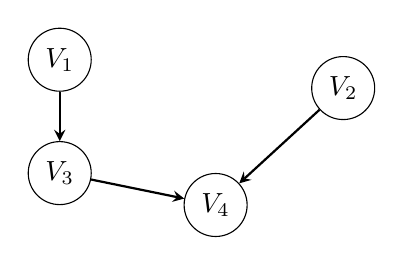
\begin{tikzpicture}[>=stealth,scale=0.9]
  \node[draw,circle,minimum size=8mm] (v1) at (0,1.6) {$V_1$};
  \node[draw,circle,minimum size=8mm] (v3) at (0,0) {$V_3$};
  \node[draw,circle,minimum size=8mm] (v4) at (2.2,-0.45) {$V_4$};
  \node[draw,circle,minimum size=8mm] (v2) at (4.0,1.2) {$V_2$};
  \draw[->,thick] (v1) -- (v3);
  \draw[->,thick] (v3) -- (v4);
  \draw[->,thick] (v2) -- (v4);
\end{tikzpicture}
\end{center}

（1）写出所有可能的拓扑序列： \blank。\\
（2）若要使该图只有唯一的拓扑序列，则可以添加一条弧 \blank。\\
\begin{solution}
拓扑序列为 $1234,1324,2134$。枚举时先列出入度为 $0$ 的顶点，每次删除一个当前入度为 $0$ 的顶点并更新后继入度；若某一步有多个入度为 $0$ 的顶点，就产生不同拓扑序列。要使拓扑序列唯一，需要消除关键分叉：添加弧 $v_2\to v_1$ 可强制 $2$ 在 $1$ 前，唯一序列为 $2134$；添加弧 $v_3\to v_2$ 可强制 $3$ 在 $2$ 前，唯一序列为 $1324$。所加弧不能造成环，否则就不再存在拓扑序列。
\end{solution}
\end{question}

\begin{question}
在快速排序中，定义一次平分的划分为 “幸运的划分”，而一次划分如果有\\
一边为空则是“不幸的划分”。假设划分的过程总是“幸运”和“不幸”交替的，\\
则该快速排序的时间复杂性为         nlogn       。\\
\begin{solution}
时间复杂性为 $O(n\log n)$。一次“幸运划分”把问题分成大约相等的两半，递归深度贡献为 $\log n$；一次“不幸划分”虽然只去掉很少元素，但题设说明幸运和不幸交替出现，因此每两层递归后问题规模仍会至少缩小为常数比例。每一层划分扫描当前子数组，所有同层子问题的扫描量合计为 $O(n)$，层数仍为 $O(\log n)$，所以总复杂度为 $O(n\log n)$，不是快速排序最坏情形的 $O(n^2)$。
\end{solution}
\end{question}

\begin{question}
具有10000 个关键码的16 阶B 树的查找路径长度（从根到叶节点访问B\\
树索引块的次数）不会小于   3    。\\
\begin{solution}
答案为 $3$。题目问“不会小于”多少，因此只需证明路径长度不可能是 $1$ 或 $2$。$16$ 阶 B 树每个结点最多 $15$ 个关键码、$16$ 个孩子。若查找路径长度按访问 B 树索引块层数计，两层最多容纳
\[
15+16\cdot15=255
\]
个关键码，远小于 $10000$，所以查找路径长度至少为 $3$。本题填空给的是下界，不要求继续判断 $3$ 层是否一定足够；若改问精确高度，还需要结合根、非根结点的最小/最大关键码数重新估计。
\end{solution}
\end{question}

\begin{question}
设有8 个初始归并段，其长度分别为32，46，56，64，20，87，70，40；\\
进行3 路归并排序，所构造的最佳归并树对应的总读写次数为 1590   。\\
\begin{solution}
最佳 3 路归并树的带权外部路径长度为 $795$，总读写次数为 $2\times795=1590$。3 路归并要求构造 3 叉 Huffman 树；因初始归并段数为 $8$，满足 $(n-1)\bmod(3-1)=1$，需补一个长度为 $0$ 的虚段，使叶子数变为 $9$。每次合并三个最短段并把新段重新放回候选集合，所有合并产生的新段长度之和就是 WPL；外排序每条记录每过一层通常读一次写一次，因此总 I/O 量为 $2WPL$。
\end{solution}
\end{question}

\begin{question}
A[N][N]是对称矩阵，现将下三角矩阵按行存储到一维数组T[N(N+1)/2]中\\
（包括对角线），则对任一上三角元素A[i][j]其对应值（0 <= i <= j < N）在\\
T[k]中的下标k 是     j(j+1)/2+i       。\\
\begin{solution}
下标为 $k=j(j+1)/2+i$，这里默认数组从 $0$ 开始编号且题中访问的是上三角元素 $A[i][j]$（$i<j$）。对称矩阵满足 $A[i][j]=A[j][i]$，而下三角按行存储时，第 $j$ 行之前共有 $0+1+\cdots+j=j(j+1)/2$ 个元素，本行中 $A[j][i]$ 的偏移为 $i$，故总下标为 $k=j(j+1)/2+i$。若采用 1 下标，公式需相应减去常数偏移。
\end{solution}
\end{question}

\begin{question}
在一棵空AVL 树中，顺序插入如下关键码：\{5, 9, 4, 2, 1, 3, 8\}，请问全部\\
插入后，在等概率下查找成功的平均检索长度为  17/7     。\\
\begin{solution}
最终 AVL 树各结点查找长度和为 $17$，等概率成功平均检索长度为 $17/7$。插入序列 $\{5,9,4,2,1,3,8\}$ 时，插入 $1$ 后在结点 $4$ 处出现 LL 型失衡，需右旋；插入 $3$ 后在相应祖先处出现 LR 型调整，先左旋再右旋；插入 $8$ 后保持平衡。按最终树从根开始把根的查找长度计为 $1$，逐层累计 7 个结点的查找长度之和为 $17$，所以平均成功查找长度为 $17/7$。
\end{solution}
\end{question}

\begin{question}
已知广义表 C=(c, (d, A), B, e)，则广义表C 的深度为   2     ，\\
tail(head(tail(C)))的运算结果为  (A)     。\\
\begin{solution}
广义表深度为 $2$；$tail(head(tail(C)))=(A)$。因为 $C=(c,(d,A),B,e)$ 的元素中只有第二个元素 $(d,A)$ 是子表，且该子表内部不再出现更深的括号，所以最大括号嵌套层数为 $2$。计算表达式时，$tail(C)=((d,A),B,e)$，$head(tail(C))=(d,A)$，再取其尾部得到 $(A)$；注意广义表的 \texttt{tail} 返回的是“去掉表头后的子表”，不是单个原子 $A$。
\end{solution}
\end{question}

\textbf{二、简答辨析题（每题3 分，共 15 分）}
\begin{question}
如果要找出一个具有n 个元素集合中的第k (1<=k<=n)个最小元素，所学过的\\
排序方法中哪种最适合？给出实现的基本思想。\\
\begin{solution}
最适合用快速选择思想。任选或随机选一个枢轴，把数组划分为“小于枢轴、等于枢轴、大于枢轴”三部分；若枢轴最终秩为 $k$，它就是第 $k$ 小元素；若枢轴秩大于 $k$，只需递归处理左侧；若枢轴秩小于 $k$，只需在右侧查找相应的新秩。与快速排序不同，快速选择每层只递归进入一边，平均递推为 $T(n)=T(n/2)+O(n)$，故平均时间为 $O(n)$，额外空间可做到 $O(1)$ 或递归栈 $O(\log n)$。
\end{solution}
\end{question}

\begin{question}
已知一组关键码为（26，36，41，38，44，15，68，12，06，51，25），散列表长度为 15，用线性探查法解决冲突构造这组关键码的散列表。散列函数为 $h(k)=k\bmod 13$。请回答：\\
(1) 构造顺序插入上述关键码集合后的散列表；\\
(2) 下一记录放到第 11 个槽和第 7 个槽中的概率分别是多少？\\
(3) 查找成功和失败情形下的平均查找长度 ASL 分别是多少？
\begin{solution}
顺序插入后散列表为：
\begin{center}
\begin{tabular}{c|ccccccccccccccc}
地址&0&1&2&3&4&5&6&7&8&9&10&11&12&13&14\\ \hline
关键码&26&25&41&15&68&44&6&--&--&--&36&--&38&12&51
\end{tabular}
\end{center}
下一记录放到第 $11$ 个槽的概率为 $2/13$，放到第 $7$ 个槽的概率为 $9/13$。查找成功的平均查找长度为 $20/11$；查找失败的平均查找长度为 $52/13=4$。
\end{solution}
\end{question}

\begin{question}
有如下图所示的一个 3 阶 B+ 树，请分别画出依次插入关键码 10 和删除关键码 4 的 B+ 树，并分析上述操作过程中的访外读写次数。
\begin{center}
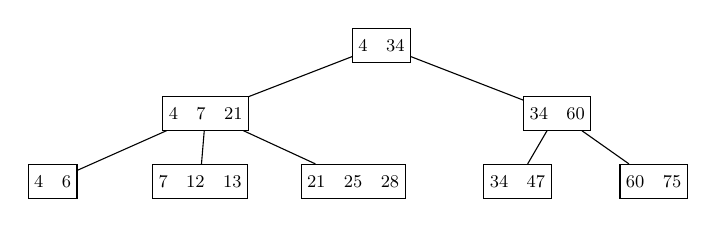
\begin{tikzpicture}[scale=0.72,transform shape]
  \tikzset{bt/.style={draw,rectangle,minimum height=6mm,inner sep=3pt,font=\small}}
  \node[bt] (r) at (5.8,3.2) {4\quad 34};
  \node[bt] (l) at (2.7,2.0) {4\quad 7\quad 21};
  \node[bt] (rr) at (8.9,2.0) {34\quad 60};
  \node[bt] (l1) at (0.0,0.8) {4\quad 6};
  \node[bt] (l2) at (2.6,0.8) {7\quad 12\quad 13};
  \node[bt] (l3) at (5.3,0.8) {21\quad 25\quad 28};
  \node[bt] (r1) at (8.2,0.8) {34\quad 47};
  \node[bt] (r2) at (10.6,0.8) {60\quad 75};
  \draw (r)--(l); \draw (r)--(rr);
  \draw (l)--(l1); \draw (l)--(l2); \draw (l)--(l3);
  \draw (rr)--(r1); \draw (rr)--(r2);
\end{tikzpicture}
\end{center}
\begin{solution}
插入 $10$ 后根结点变为 $[4,12,34]$，对应叶结点分裂为 $[4,6]$、$[7,10]$、$[12,13]$、$[21,25,28]$、$[34,47]$、$[60,75]$，读 $3$ 次、写 $5$ 次：
\begin{center}
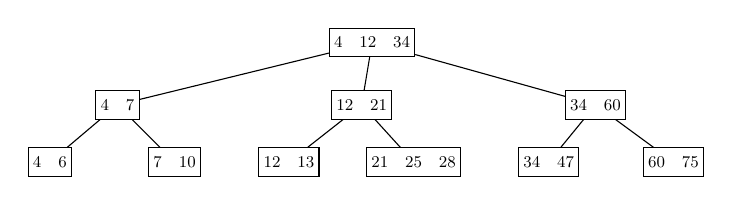
\begin{tikzpicture}[scale=0.66,transform shape]
  \tikzset{bt/.style={draw,rectangle,minimum height=5.5mm,inner sep=2.6pt,font=\small}}
  \node[bt] (r) at (6.2,3.0) {4\quad 12\quad 34};
  \node[bt] (a) at (1.3,1.8) {4\quad 7};
  \node[bt] (b) at (6.0,1.8) {12\quad 21};
  \node[bt] (c) at (10.5,1.8) {34\quad 60};
  \node[bt] (a1) at (0.0,0.7) {4\quad 6};
  \node[bt] (a2) at (2.4,0.7) {7\quad 10};
  \node[bt] (b1) at (4.6,0.7) {12\quad 13};
  \node[bt] (b2) at (7.0,0.7) {21\quad 25\quad 28};
  \node[bt] (c1) at (9.6,0.7) {34\quad 47};
  \node[bt] (c2) at (12.0,0.7) {60\quad 75};
  \draw (r)--(a); \draw (r)--(b); \draw (r)--(c);
  \draw (a)--(a1); \draw (a)--(a2);
  \draw (b)--(b1); \draw (b)--(b2);
  \draw (c)--(c1); \draw (c)--(c2);
\end{tikzpicture}
\end{center}
删除 $4$ 后根结点为 $[6,34]$，左内部结点为 $[6,12,21]$，右内部结点为 $[34,60]$，写 $3$ 次：
\begin{center}
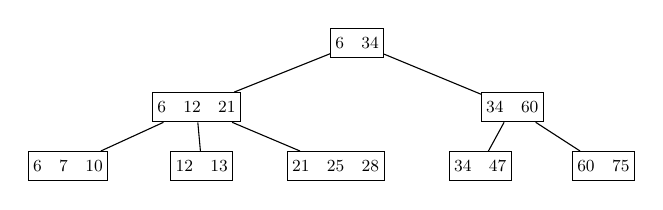
\begin{tikzpicture}[scale=0.68,transform shape]
  \tikzset{bt/.style={draw,rectangle,minimum height=5.5mm,inner sep=2.6pt,font=\small}}
  \node[bt] (r) at (5.4,3.0) {6\quad 34};
  \node[bt] (a) at (2.4,1.8) {6\quad 12\quad 21};
  \node[bt] (b) at (8.3,1.8) {34\quad 60};
  \node[bt] (a1) at (0.0,0.7) {6\quad 7\quad 10};
  \node[bt] (a2) at (2.5,0.7) {12\quad 13};
  \node[bt] (a3) at (5.0,0.7) {21\quad 25\quad 28};
  \node[bt] (b1) at (7.7,0.7) {34\quad 47};
  \node[bt] (b2) at (10.0,0.7) {60\quad 75};
  \draw (r)--(a); \draw (r)--(b);
  \draw (a)--(a1); \draw (a)--(a2); \draw (a)--(a3);
  \draw (b)--(b1); \draw (b)--(b2);
\end{tikzpicture}
\end{center}
\end{solution}
\end{question}

\begin{question}
一棵红黑树如下图所示（空树叶未画出），请首先画出插入节点 17 的红黑树，在此基础上，然后画出删除节点 14 的红黑树。（画图说明：黑节点用方框，红节点用圆圈，不画空树叶。）
\begin{center}
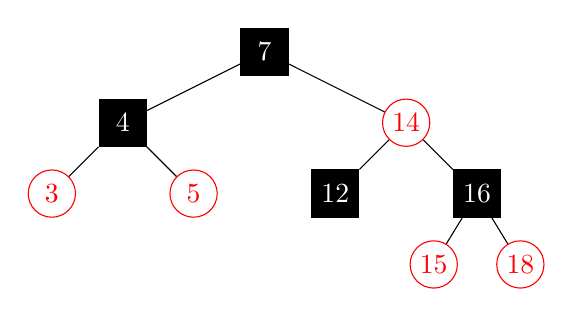
\begin{tikzpicture}[level distance=9mm,
  blacknode/.style={draw,rectangle,fill=black,text=white,minimum size=6mm,inner sep=1pt},
  rednode/.style={draw,circle,red,text=red,minimum size=6mm,inner sep=1pt},
  level 1/.style={sibling distance=36mm},
  level 2/.style={sibling distance=18mm},
  level 3/.style={sibling distance=11mm}]
\node[blacknode] {7}
  child {node[blacknode] {4}
    child {node[rednode] {3}}
    child {node[rednode] {5}}}
  child {node[rednode] {14}
    child {node[blacknode] {12}}
    child {node[blacknode] {16}
      child {node[rednode] {15}}
      child {node[rednode] {18}}}};
\end{tikzpicture}
\end{center}
\begin{solution}
插入 $17$ 后：
\begin{center}
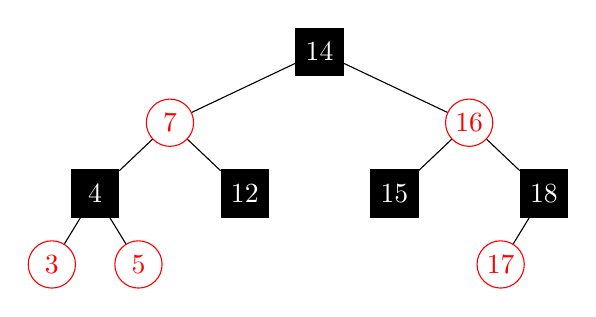
\begin{tikzpicture}[level distance=9mm,
  blacknode/.style={draw,rectangle,fill=black,text=white,minimum size=6mm,inner sep=1pt},
  rednode/.style={draw,circle,red,text=red,minimum size=6mm,inner sep=1pt},
  level 1/.style={sibling distance=38mm},
  level 2/.style={sibling distance=19mm},
  level 3/.style={sibling distance=11mm}]
\node[blacknode] {14}
  child {node[rednode] {7}
    child {node[blacknode] {4}
      child {node[rednode] {3}}
      child {node[rednode] {5}}}
    child {node[blacknode] {12}}}
  child {node[rednode] {16}
    child {node[blacknode] {15}}
    child {node[blacknode] {18}
      child {node[rednode] {17}}
      child[missing]}};
\end{tikzpicture}
\end{center}
继续删除 $14$ 后：
\begin{center}
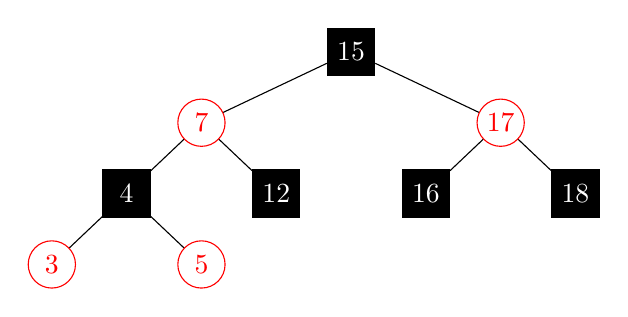
\begin{tikzpicture}[level distance=9mm,
  blacknode/.style={draw,rectangle,fill=black,text=white,minimum size=6mm,inner sep=1pt},
  rednode/.style={draw,circle,red,text=red,minimum size=6mm,inner sep=1pt},
  level 1/.style={sibling distance=38mm},
  level 2/.style={sibling distance=19mm}]
\node[blacknode] {15}
  child {node[rednode] {7}
    child {node[blacknode] {4}
      child {node[rednode] {3}}
      child {node[rednode] {5}}}
    child {node[blacknode] {12}}}
  child {node[rednode] {17}
    child {node[blacknode] {16}}
    child {node[blacknode] {18}}};
\end{tikzpicture}
\end{center}
\end{solution}
\end{question}

\begin{question}
字符串的后缀是指字符串的任意尾部串。比如 “abbc” 的后缀有 “abbc”，“bbc”，“bc”，“c” 和 \texttt{\$}（表示为空串）。现有两个字符串 “window” 和 “indigo”，请画出它们所有后缀串所组成的 Trie 树（注意：对路径进行压缩，并把局部子串标注在相应的边上）。
\begin{solution}
压缩 Trie 可按首字符分支；叶结点标注 $(s,i)$ 表示第 $s$ 个字符串从下标 $i$ 开始的后缀，其中 $1$ 表示 \texttt{window\$}，$2$ 表示 \texttt{indigo\$}。
\begin{center}
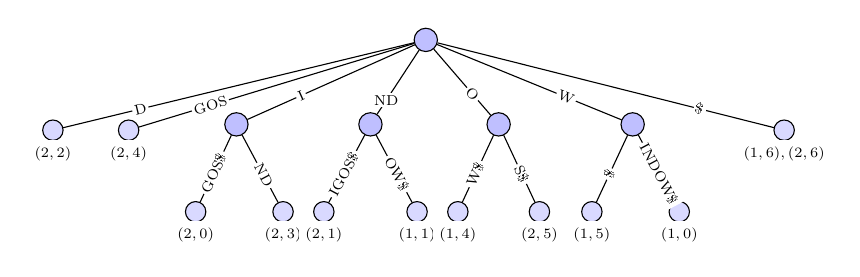
\begin{tikzpicture}[>=stealth,scale=0.74,transform shape,
  inner/.style={draw,circle,fill=blue!25,minimum size=4mm,inner sep=0.5pt},
  leaf/.style={draw,circle,fill=blue!15,minimum size=3.5mm,inner sep=0.5pt},
  lab/.style={draw=none,fill=white,inner sep=1pt,font=\scriptsize}]
  \node[inner] (r) at (0,0) {};
  \node[leaf] (d) at (-6.4,-1.55) {};
  \node[leaf] (g1) at (-5.1,-1.55) {};
  \node[inner] (i) at (-3.25,-1.45) {};
  \node[leaf] (ig0) at (-3.95,-2.95) {};
  \node[leaf] (ig1) at (-2.45,-2.95) {};
  \node[inner] (n) at (-0.95,-1.45) {};
  \node[leaf] (n1) at (-1.75,-2.95) {};
  \node[leaf] (n2) at (-0.15,-2.95) {};
  \node[inner] (o) at (1.25,-1.45) {};
  \node[leaf] (o1) at (0.55,-2.95) {};
  \node[leaf] (o2) at (1.95,-2.95) {};
  \node[inner] (w) at (3.55,-1.45) {};
  \node[leaf] (w1) at (2.85,-2.95) {};
  \node[leaf] (w2) at (4.35,-2.95) {};
  \node[leaf] (dol) at (6.15,-1.55) {};
  \draw (r)--node[lab,sloped,pos=.78]{D}(d);
  \draw (r)--node[lab,sloped,pos=.74]{GOS}(g1);
  \draw (r)--node[lab,sloped,pos=.68]{I}(i);
  \draw (i)--node[lab,sloped,pos=.56]{GOS\$}(ig0);
  \draw (i)--node[lab,sloped,pos=.60]{ND}(ig1);
  \draw (r)--node[lab,pos=.78]{ND}(n);
  \draw (n)--node[lab,sloped,pos=.58]{IGOS\$}(n1);
  \draw (n)--node[lab,sloped,pos=.58]{OW\$}(n2);
  \draw (r)--node[lab,sloped,pos=.68]{O}(o);
  \draw (o)--node[lab,sloped,pos=.58]{W\$}(o1);
  \draw (o)--node[lab,sloped,pos=.58]{S\$}(o2);
  \draw (r)--node[lab,sloped,pos=.70]{W}(w);
  \draw (w)--node[lab,sloped,pos=.58]{\$}(w1);
  \draw (w)--node[lab,sloped,pos=.58]{INDOW\$}(w2);
  \draw (r)--node[lab,sloped,pos=.78]{\$}(dol);
  \node[draw=none,fill=white,font=\scriptsize] at (-6.4,-1.95) {$(2,2)$};
  \node[draw=none,fill=white,font=\scriptsize] at (-5.1,-1.95) {$(2,4)$};
  \node[draw=none,fill=white,font=\scriptsize] at (-3.95,-3.35) {$(2,0)$};
  \node[draw=none,fill=white,font=\scriptsize] at (-2.45,-3.35) {$(2,3)$};
  \node[draw=none,fill=white,font=\scriptsize] at (-1.75,-3.35) {$(2,1)$};
  \node[draw=none,fill=white,font=\scriptsize] at (-0.15,-3.35) {$(1,1)$};
  \node[draw=none,fill=white,font=\scriptsize] at (0.55,-3.35) {$(1,4)$};
  \node[draw=none,fill=white,font=\scriptsize] at (1.95,-3.35) {$(2,5)$};
  \node[draw=none,fill=white,font=\scriptsize] at (2.85,-3.35) {$(1,5)$};
  \node[draw=none,fill=white,font=\scriptsize] at (4.35,-3.35) {$(1,0)$};
  \node[draw=none,fill=white,font=\scriptsize] at (6.15,-1.95) {$(1,6),(2,6)$};
\end{tikzpicture}
\end{center}
\end{solution}
\end{question}

\textbf{三、算法填空题（每空1 分，共5 分）}
\begin{question}
下述算法实现在图G 中计算从顶点i 到顶点j 之间长度为len 的简单路径条\\
数。图的ADT 如下：
\begin{pycode}
class Graph:
    def first_edge(self, vertex): ...
    def next_edge(self, edge): ...
    def is_edge(self, edge): ...
    def to_vertex(self, edge): ...


visited = [False] * MAXSIZE


def get_path_num_len(G, i, j, length):
    if i == j and length == 0:
        return 1

    total = 0
    visited[i] = True
    e = G.first_edge(i)
    while G.is_edge(e):
        v = G.to_vertex(e)
        if not visited[v]:
            total += get_path_num_len(G, v, j, length - 1)
        e = G.next_edge(e)

    visited[i] = False
    return total
\end{pycode}

\begin{solution}
填空为 \texttt{\detokenize{i == j and length == 0}}；递归累加语句为 \texttt{\detokenize{total += get_path_num_len(G, v, j, length - 1)}}。递归的出口表示“已经走完规定长度”，只有此时当前位置正好是终点 $j$ 才返回 $1$。否则枚举当前顶点 $i$ 的每个未访问邻接点 $v$，把问题化为从 $v$ 到 $j$、剩余长度为 $length-1$ 的路径条数。为保证路径简单，进入递归前后要正确设置和恢复访问标记。
\end{solution}
\end{question}

\begin{question}
下面的代码实现了一种计数排序：对每个待排序记录，扫描整个序列统计\\
比它小的记录个数count，count 即是该记录在序列中的争取位置。请将下\\
面是计数排序的程序代码补充完整。
\begin{pycode}
def sort_records(array):
    cur_index = 0              # 待排下标
    n = len(array)
    while cur_index < n:
        count = 0
        for j in range(n):     # 统计比 array[cur_index] 小的值的个数
            if array[j] < array[cur_index]:
                count += 1

        array[cur_index], array[count] = array[count], array[cur_index]
        if cur_index == count:
            cur_index += 1
    return array
\end{pycode}

\begin{solution}
填空为统计所有小于当前记录的元素个数 $count$，将当前记录交换到 $count$ 位置；若当前位置已经正确则推进 $curIndex$。该算法需注意重复关键码时要用稳定计数或额外规则处理。
\end{solution}
\end{question}

\textbf{四、设计分析题（共 9 分）}
\begin{question}
（3 分）某小区有N 座别墅需要供水。在第i 座别墅里挖井需要w[i]的费用，\\
在第i 座和第j 座别墅之间铺水管需要c[i][j]的费用。给每座别墅供水，要\\
么挖井、要么跟其他有井的别墅铺设连通的水管路径。请设计算法，求解\\
使每座别墅都得到供水的最小费用方案。\\
\begin{solution}
构造一个额外水源顶点 $s$。从 $s$ 到第 $i$ 座别墅连一条边，权重为 $w[i]$，表示“在第 $i$ 座别墅挖井”；别墅 $i,j$ 之间连边权重为 $c[i][j]$，表示铺设两者之间的管道。这样，任何让所有别墅有水的方案都对应于扩展图中连接 $s$ 和全部别墅的一棵连通子图；去掉其中的环不会增加费用，所以最优方案一定是一棵生成树。对该图求最小生成树，选中的 $s-i$ 边表示挖井，选中的别墅间边表示铺管，即为最小费用供水方案。
\end{solution}
\end{question}

\begin{question}
（6 分）现有一个工资系统，请实现满足如下操作需求的Splay 树，并给出\\
算法的伪代码：（Splay 树根为root，其他变量可以自己定义）\\
1) \texttt{\detokenize{insert(w)}}：新加一位工资为 $w$ 的员工（假设 $w$ 没有重复值）；\\
2) \texttt{\detokenize{fire(t)}}：解雇工资大于 $t$ 的员工。\\
相关定义和函数说明如下：\\
伸展树是一种自平衡的 BST，数据结构如下：
\begin{pycode}
class TreeNode:
    def __init__(self, wage):
        self.wage = wage
        self.father = None
        self.left = None
        self.right = None
\end{pycode}
可以直接使用的函数：
\begin{pycode}
def Splay(x, f):
    """将 x 旋转为 f 的子结点；f 为 None 时把 x 旋到根。"""


def find(x, subtree):
    """在 subtree 中查找 x；若失败，返回 x 应插入位置的父结点。"""


def Delete(x):
    """删除以 x 为根的子树。"""


root = None


def insert(w):
    global root
    if root is None:
        root = TreeNode(w)
        return

    parent = find(w, root)
    new_node = TreeNode(w)
    new_node.father = parent
    if w < parent.wage:
        parent.left = new_node
    else:
        parent.right = new_node
    Splay(new_node, None)
    root = new_node


def fire(t):
    global root
    if root is None:
        return

    boundary = find(t, root)
    if boundary.wage == t:
        Splay(boundary, None)
        Delete(boundary.right)
        boundary.right = None
        root = boundary
        return

    parent = boundary
    sentinel = TreeNode(t)
    sentinel.father = parent
    if t < parent.wage:
        parent.left = sentinel
    else:
        parent.right = sentinel

    Splay(sentinel, None)
    Delete(sentinel.right)
    root = sentinel.left
    if root is not None:
        root.father = None
\end{pycode}

\begin{solution}
插入时按 BST 规则定位工资 $w$ 的插入父结点，挂接新结点后将新结点 splay 到根。解雇工资大于 $t$ 的员工时，先把分界工资 $t$ 或其应插入位置伸展到根，再删除根右侧所有大于 $t$ 的子树；若临时插入了分界结点，最后删除该临时结点并恢复左右子树。
\end{solution}
\end{question}

\textbf{五、期中考试题（共25 分，成绩由助教登记）}
\textbf{六、上机考试题（共35 分，成绩由助教登记）}
